\documentclass{beamer}

%%%%%%%%%%%%%Solarized Theme%%%%%%%%%%%%%%%
\usecolortheme[dark,accent=cyan]{solarized}
\beamertemplatenavigationsymbolsempty
%%%%%Packages%%%%%
\usefonttheme{serif}
\usepackage[T1]{fontenc}
\usepackage[utf8]{inputenc}
\usepackage[english]{babel}
\usepackage{fontawesome}
\usepackage{minted}

\definecolor{DarkGray}{gray}{0.1}
\usemintedstyle{paraiso-dark}


\usepackage{graphicx}
\usepackage{hyperref}
\usepackage{colortbl, xcolor}
\usepackage{booktabs}
\usepackage{amsmath,amsthm, amssymb, latexsym}

\usepackage{tikz}
\usepackage{standalone}
\usepackage{siunitx}
\usetikzlibrary{calc, positioning, arrows, arrows.meta, shapes, automata}
\usetikzlibrary{backgrounds, fit}
\makeatletter
\newcommand{\srcsize}{\@setfontsize{\srcsize}{5pt}{5pt}}
\makeatother

\tikzstyle{arrow} = [thick,->,>=stealth]

\begin{document}

\begin{frame}
    \begin{center}
        \LARGE{\textbf{\textcolor{orange}{A bibliometric study of a research field}}} \\

        \vspace{1.5cm}
        \normalsize{PyData UK}

        \vspace{1cm}
        \normalsize{@NikoletaGlyn}

    \end{center}
\end{frame}

\begin{frame}
    \begin{center}
    
\includegraphics[width=0.24\textwidth]{static/cardiff_uni_logo.png}\hspace{6pt}
    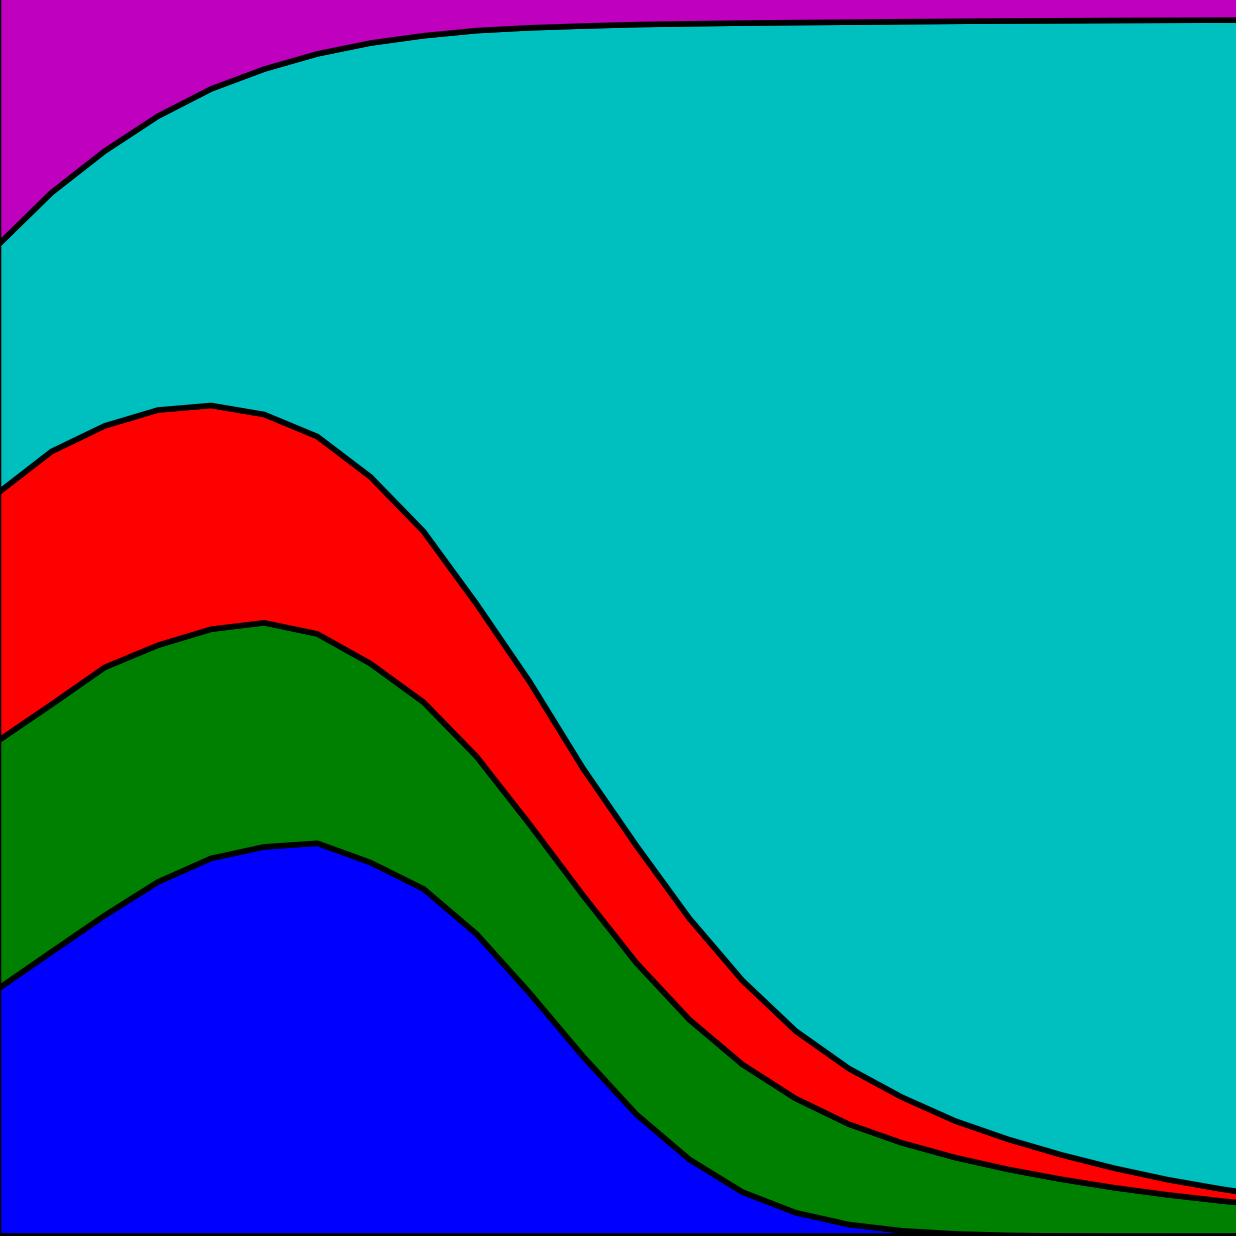
\includegraphics[width=0.24\textwidth, height=0.245\textwidth]{static/axelrod-logo.png}\vspace{10pt}

    
\includegraphics[width=0.24\textwidth]{static/ssi-logo.png} \hspace{6pt}
    
\includegraphics[width=0.24\textwidth]{static/django_girls.png}

    \end{center}
\end{frame}

\begin{frame}
    \begin{center}
    \begin{tikzpicture}

    \draw[thick] (0, 0) circle (3cm);
    \draw[solarizedGreen, fill=solarizedGreen] (0, 0) circle (0.5cm);
    \draw[line width=1mm, orange](0, 0) circle (0.8);
    \draw [arrow, line width=0.5mm, solarizedRed!70] (0.5, 0.7) -- (0.7, 1);
    \draw [arrow, line width=0.5mm, solarizedRed!40] (0.5, 0.7) -- (0.7, 1);
    \draw [arrow, line width=0.5mm, solarizedRed!60] (0.7, 1) -- (.95, 1.4);

    \draw [arrow, line width=0.5mm, red!80] (0.95, 1.4) -- (1.67, 2.5);

    \end{tikzpicture} \\ \vspace{.5cm}
    \footnotesize{\url{http://matt.might.net/articles/phd-school-in-pictures/}}
    \end{center}
\end{frame}

\begin{frame}
    \begin{center}
    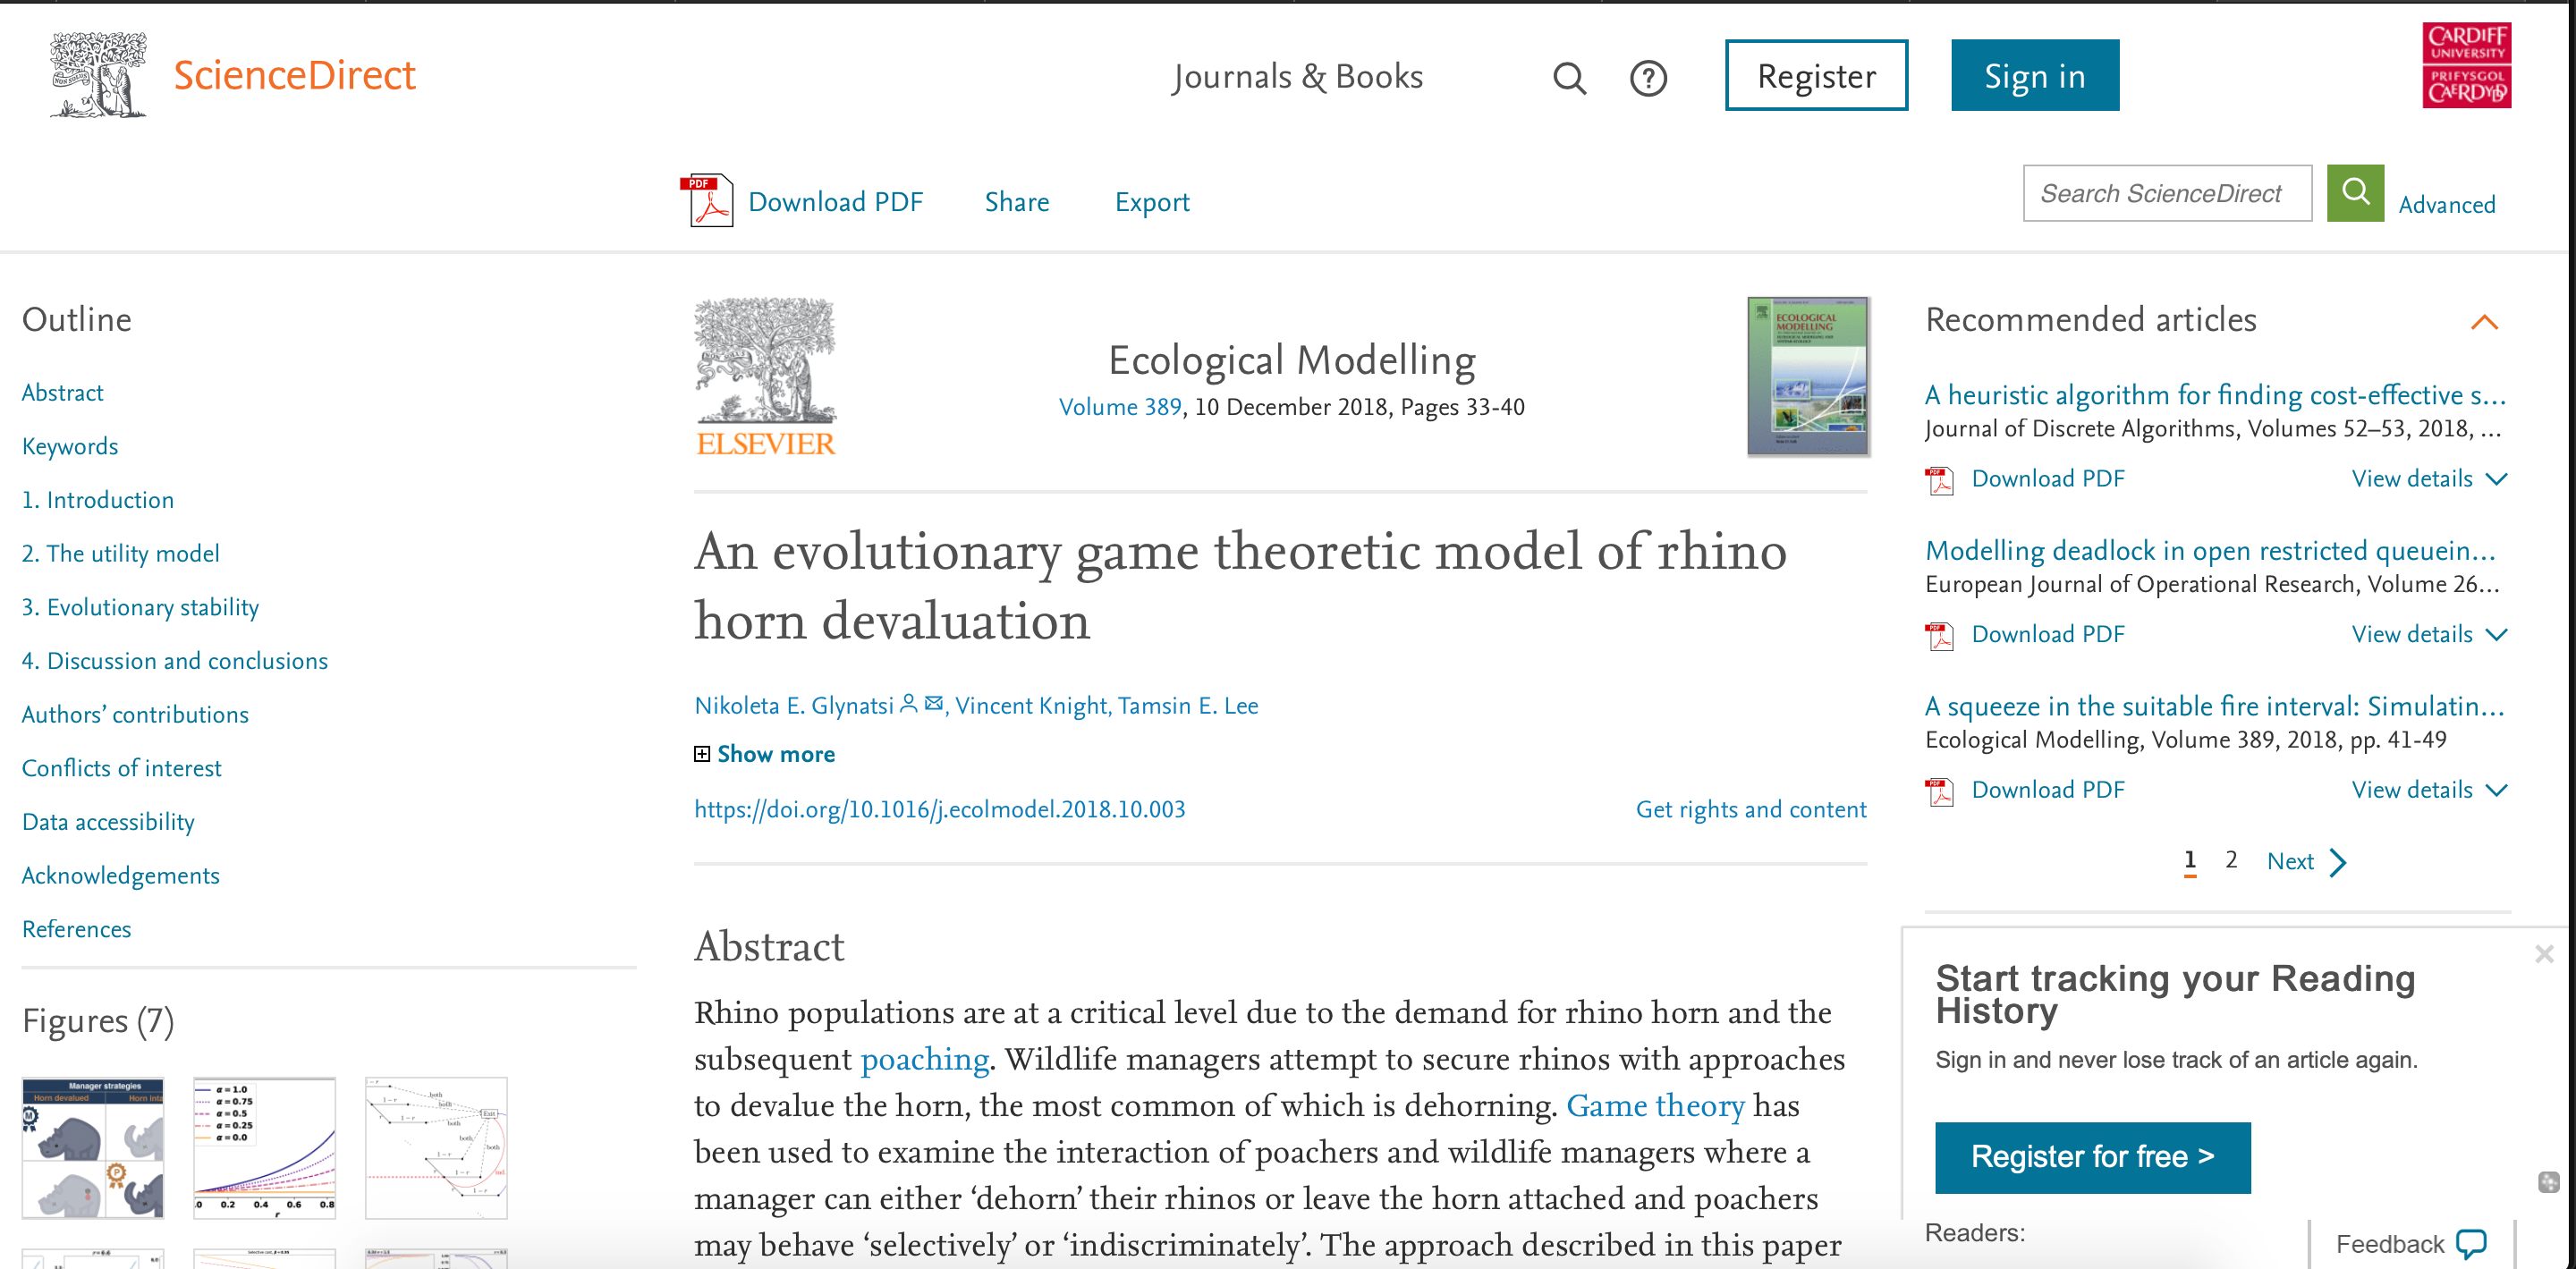
\includegraphics[width=\textwidth]{static/paper_example.png}
    \end{center}
\end{frame}

\begin{frame}
    \begin{center}
    \includestandalone{static/apis_diagram}
    \end{center}
\end{frame}

\begin{frame}
    \begin{center}
        \includestandalone{static/arcas_diagram}
    \end{center}
\end{frame}

\begin{frame}[fragile]
	\begin{minted}
    [
    framesep=4mm,
    baselinestretch=1.2,
    bgcolor=DarkGray,
    fontsize=\tiny,
    ]
    {python}
>>> import arcas
>>> plos = arcas.Plos()
>>> parameters = plos.parameters_fix(title="Game", abstract="Game", records=1, start=1)
>>> url = plos.create_url_search(parameters)
>>> url
'http://api.plos.org/search?q=title:"Game"+AND+abstract:"Game"&rows=1&start=1'
\end{minted}
\pause

\begin{minted}
    [
    framesep=4mm,
    baselinestretch=1.2,
    bgcolor=DarkGray,
    fontsize=\tiny,
    ]
    {python}
>>> request = plos.make_request(url)
>>> root = plos.get_root(request)
>>> plos_article = plos.parse(root)
[{'id': '10.1371/journal.pone.0058546',
  'journal': 'PLoS ONE',
  'eissn': '1932-6203',
  'publication_date': '2013-03-13T00:00:00Z',
  'article_type': 'Research Article',
  'author_display': ['Adam C. Oei', 'Michael D. Patterson'],
  'abstract': ['Background: Previous evidence points to ...'],
  'title_display': 'Enhancing Cognition with Video Games: A Multiple Game Training Study',
  'score': 20.51807}]
    \end{minted}
\end{frame}

\begin{frame}
    \begin{center}
    \small{title="prisoner's dilemma" OR abstract="prisoner's dilemma"}\\
    
    \vspace{-.50cm}
    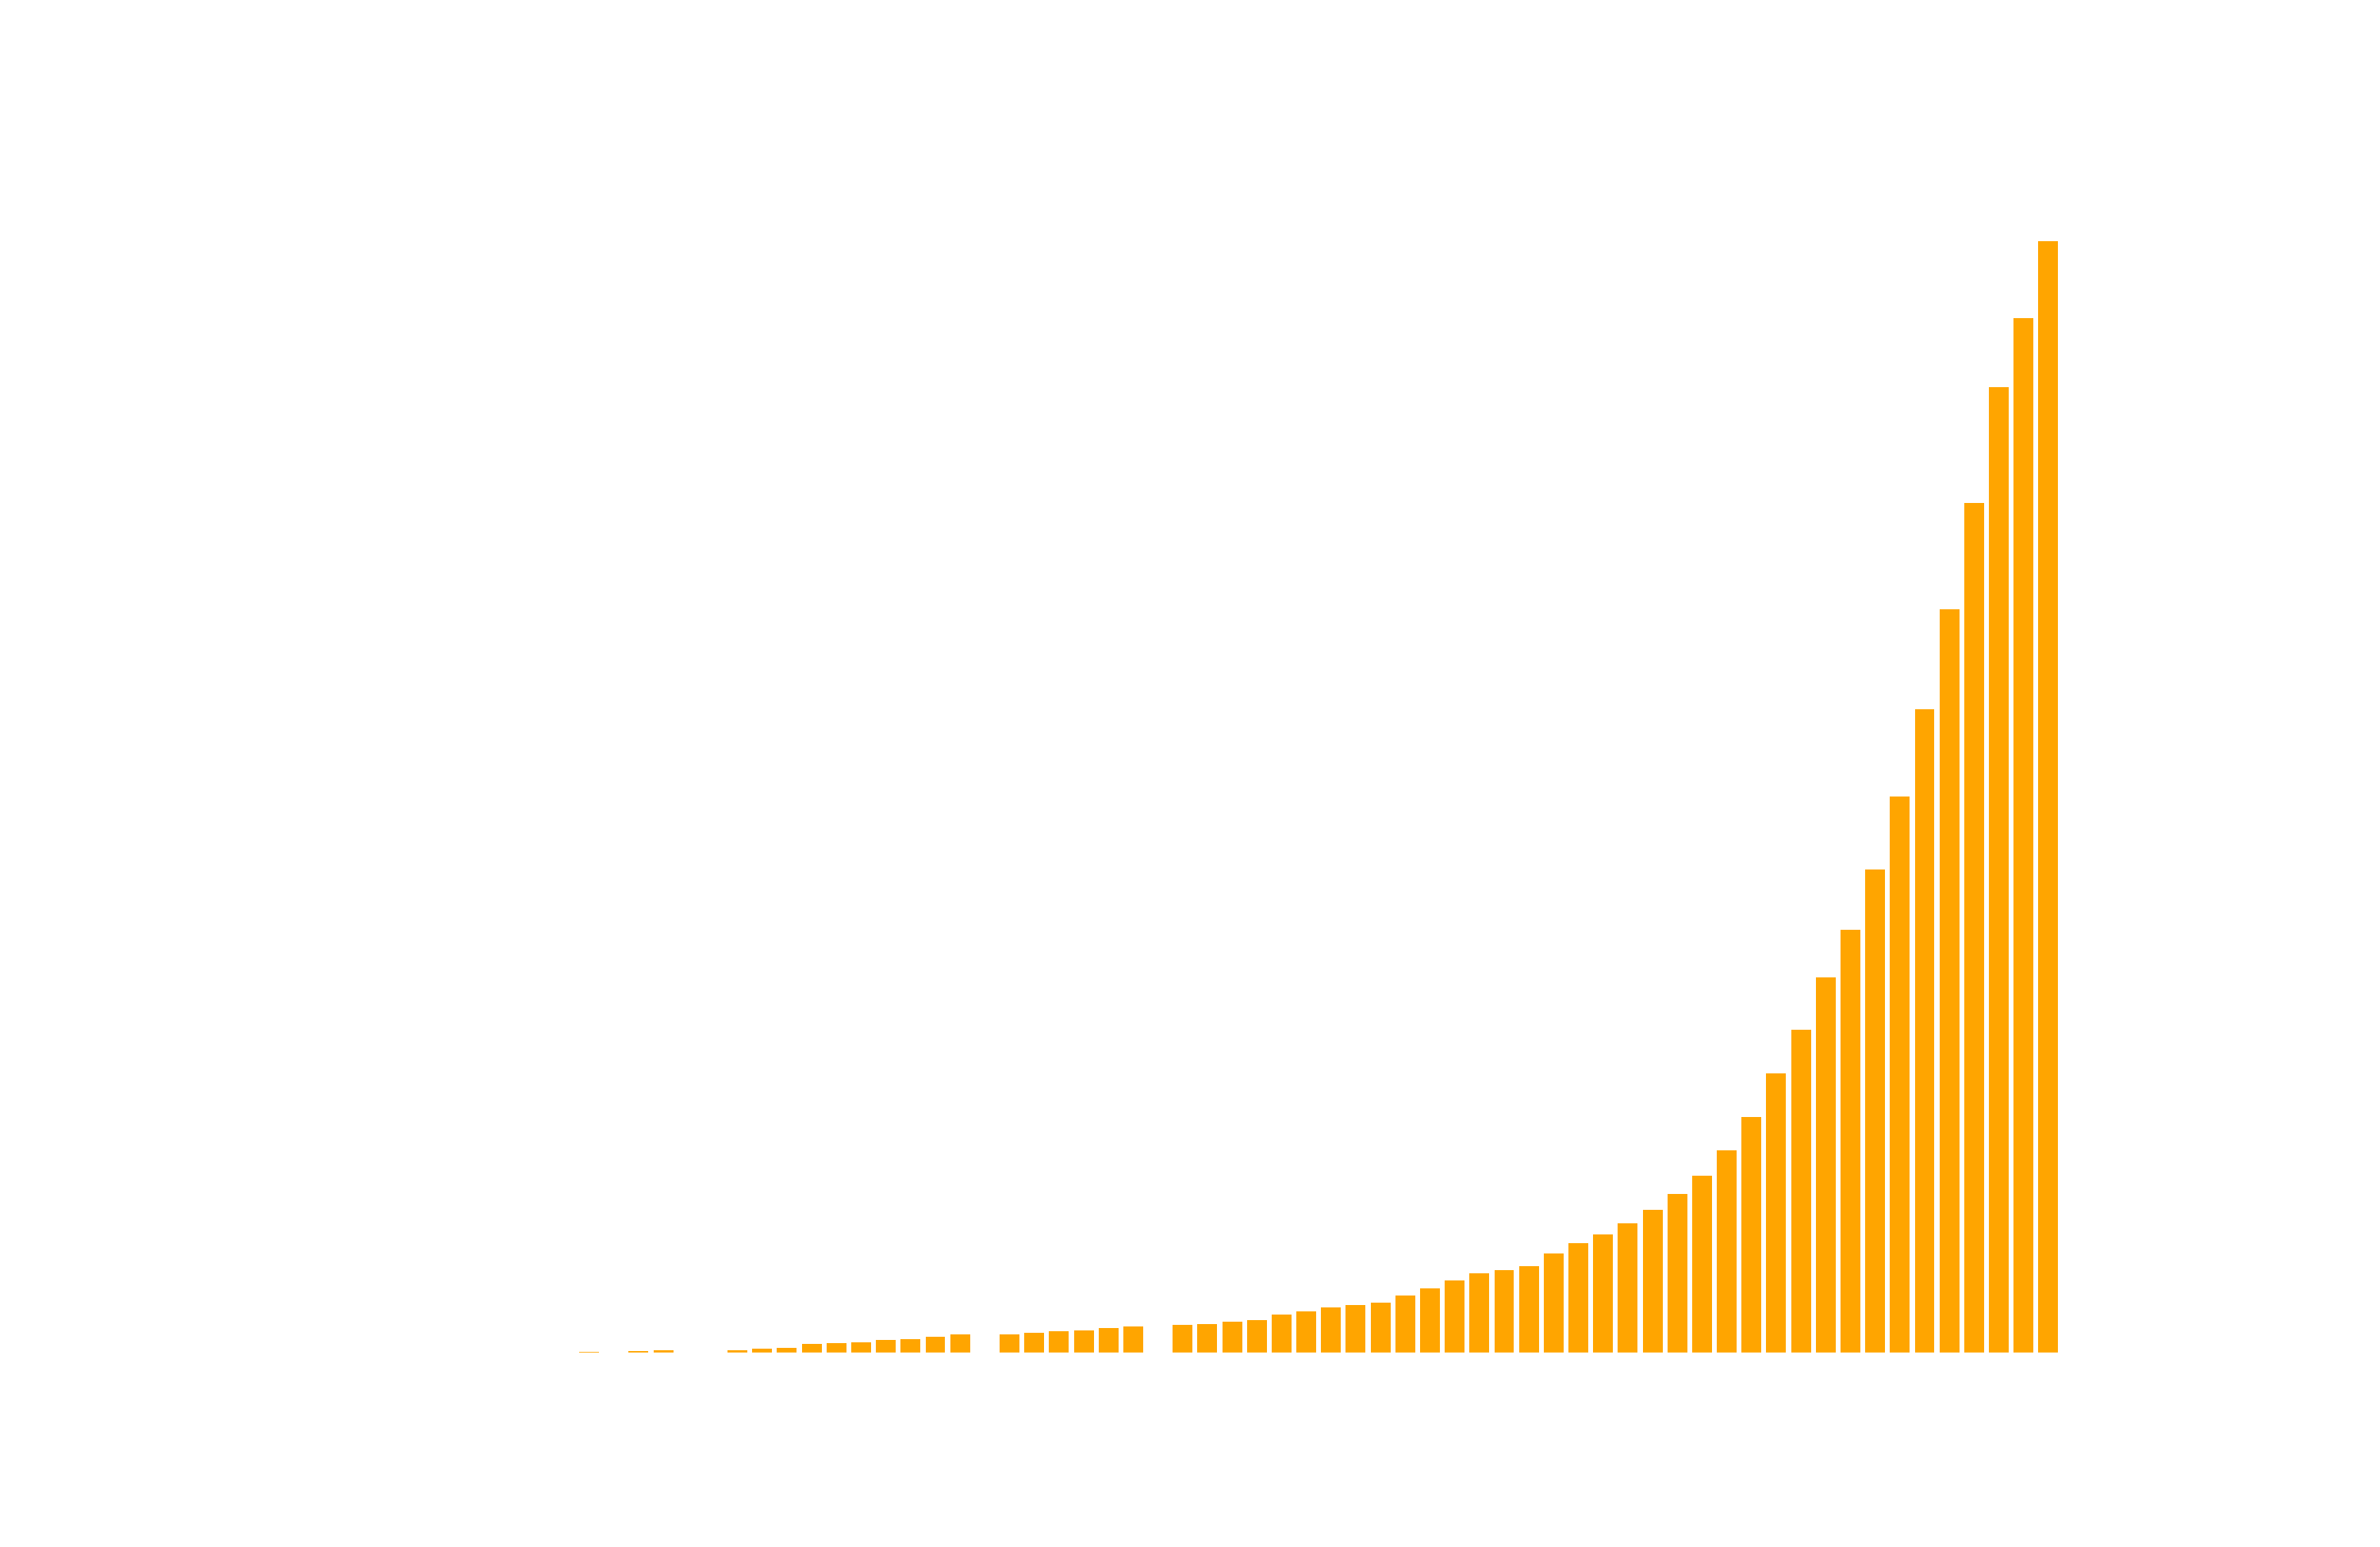
\includegraphics[width=\textwidth]{static/articles.png}
    \end{center}
\end{frame}

\begin{frame}
    \begin{center}
        \Large{\textbf{What do people write about on field of the Prisoner's Dilemma?}} \\ \vspace{1cm}
        
\includegraphics[width=.15\textwidth]{static/detective.png} \\ \vspace{.5cm}
    \end{center}
\end{frame}

\begin{frame}
    \begin{center}
        \Large{\textbf{Latent Dirichlet allocation}}
    \end{center}
\end{frame}

\begin{frame}
    \begin{center}
    
\includegraphics[width=.10\textwidth]{static/paper.png}
    
\includegraphics[width=.10\textwidth]{static/paper.png}
    
\includegraphics[width=.10\textwidth]{static/paper.png}
    
\includegraphics[width=.10\textwidth]{static/paper.png}
    \vspace{1cm}


    \resizebox{.5\textwidth}{!}{
    \begin{tabular}{lcc}
        \toprule
             & Topic 1 & Topic 2 \\
        \midrule
        "game"       & 0.200 & 0.220 \\
        "agent"      & 0.009 & 0.008 \\
        "network"    & 0.011 & 0.012 \\
        "strategy"   & 0.007 & 0.028 \\
        "population" & -     & 0.008 \\
        "social"     & 0.010 & - \\
        \bottomrule
    \end{tabular}}\vspace{1cm}
    \end{center}
\end{frame}

\begin{frame}
    \begin{center}
    abstract = ``The social network of agents'' \\ \vspace{1.5cm}

    \pause
    \(c^1\) = 0.009 + 0.011 + 0.010 = 0.30\\ 
    \(c^2\) = 0.008 + 0.012 = 0.20\\ 
    \end{center}
\end{frame}

\begin{frame}
    \begin{center}
    \begin{tikzpicture}

    \node (words) at (0, 0) {
\includegraphics[width=.15\textwidth]{static/paper.png}};

    \node[right=1cm of words] (six) {\([0.3, 0.2]\)};
    \node (dummy_out) at (1, 0) {};
    \node (dummy_in) at (2, 0) {};
    \draw (dummy_out) edge[->, out=0, in=180, draw=orange] node[above] {} (dummy_in);
    \end{tikzpicture}
    \end{center}
\end{frame}

\begin{frame}
    \begin{center}
    
\includegraphics[width=.8\textwidth]{static/coherence.png}
    \end{center}
\end{frame}

\begin{frame}
    \begin{center}
        \includestandalone{static/topics}
    \end{center}
\end{frame}

% \begin{frame}
%     \begin{center}
%     \begin{tikzpicture}

%     \node (words) at (0, 0) {
\includegraphics[width=.15\textwidth]{static/paper.png}};

%     \pause
%     \node[right=2cm of words] (six) {\LARGE{\(\mathbb{R}^5\)}};
%     \node (dummy_out) at (1.5, 0) {};
%     \node (dummy_in) at (3, 0) {};
%     \draw (dummy_out) edge[->, out=0, in=180, draw=orange] node[above] {\small{LDA}} (dummy_in);
    
%     \pause
%     \node[right=1cm of six] (two) {\Large{Topic$_i$}};
%     \node (dummy_out) at (3.7, 0) {};
%     \node (dummy_in) at (5, 0) {};
%     \draw (dummy_out) edge[->, out=0, in=180, draw=orange] node[above] {} (dummy_in);

%     \end{tikzpicture}
%     \end{center}
% \end{frame}

% \begin{frame}
%     \begin{center}
%     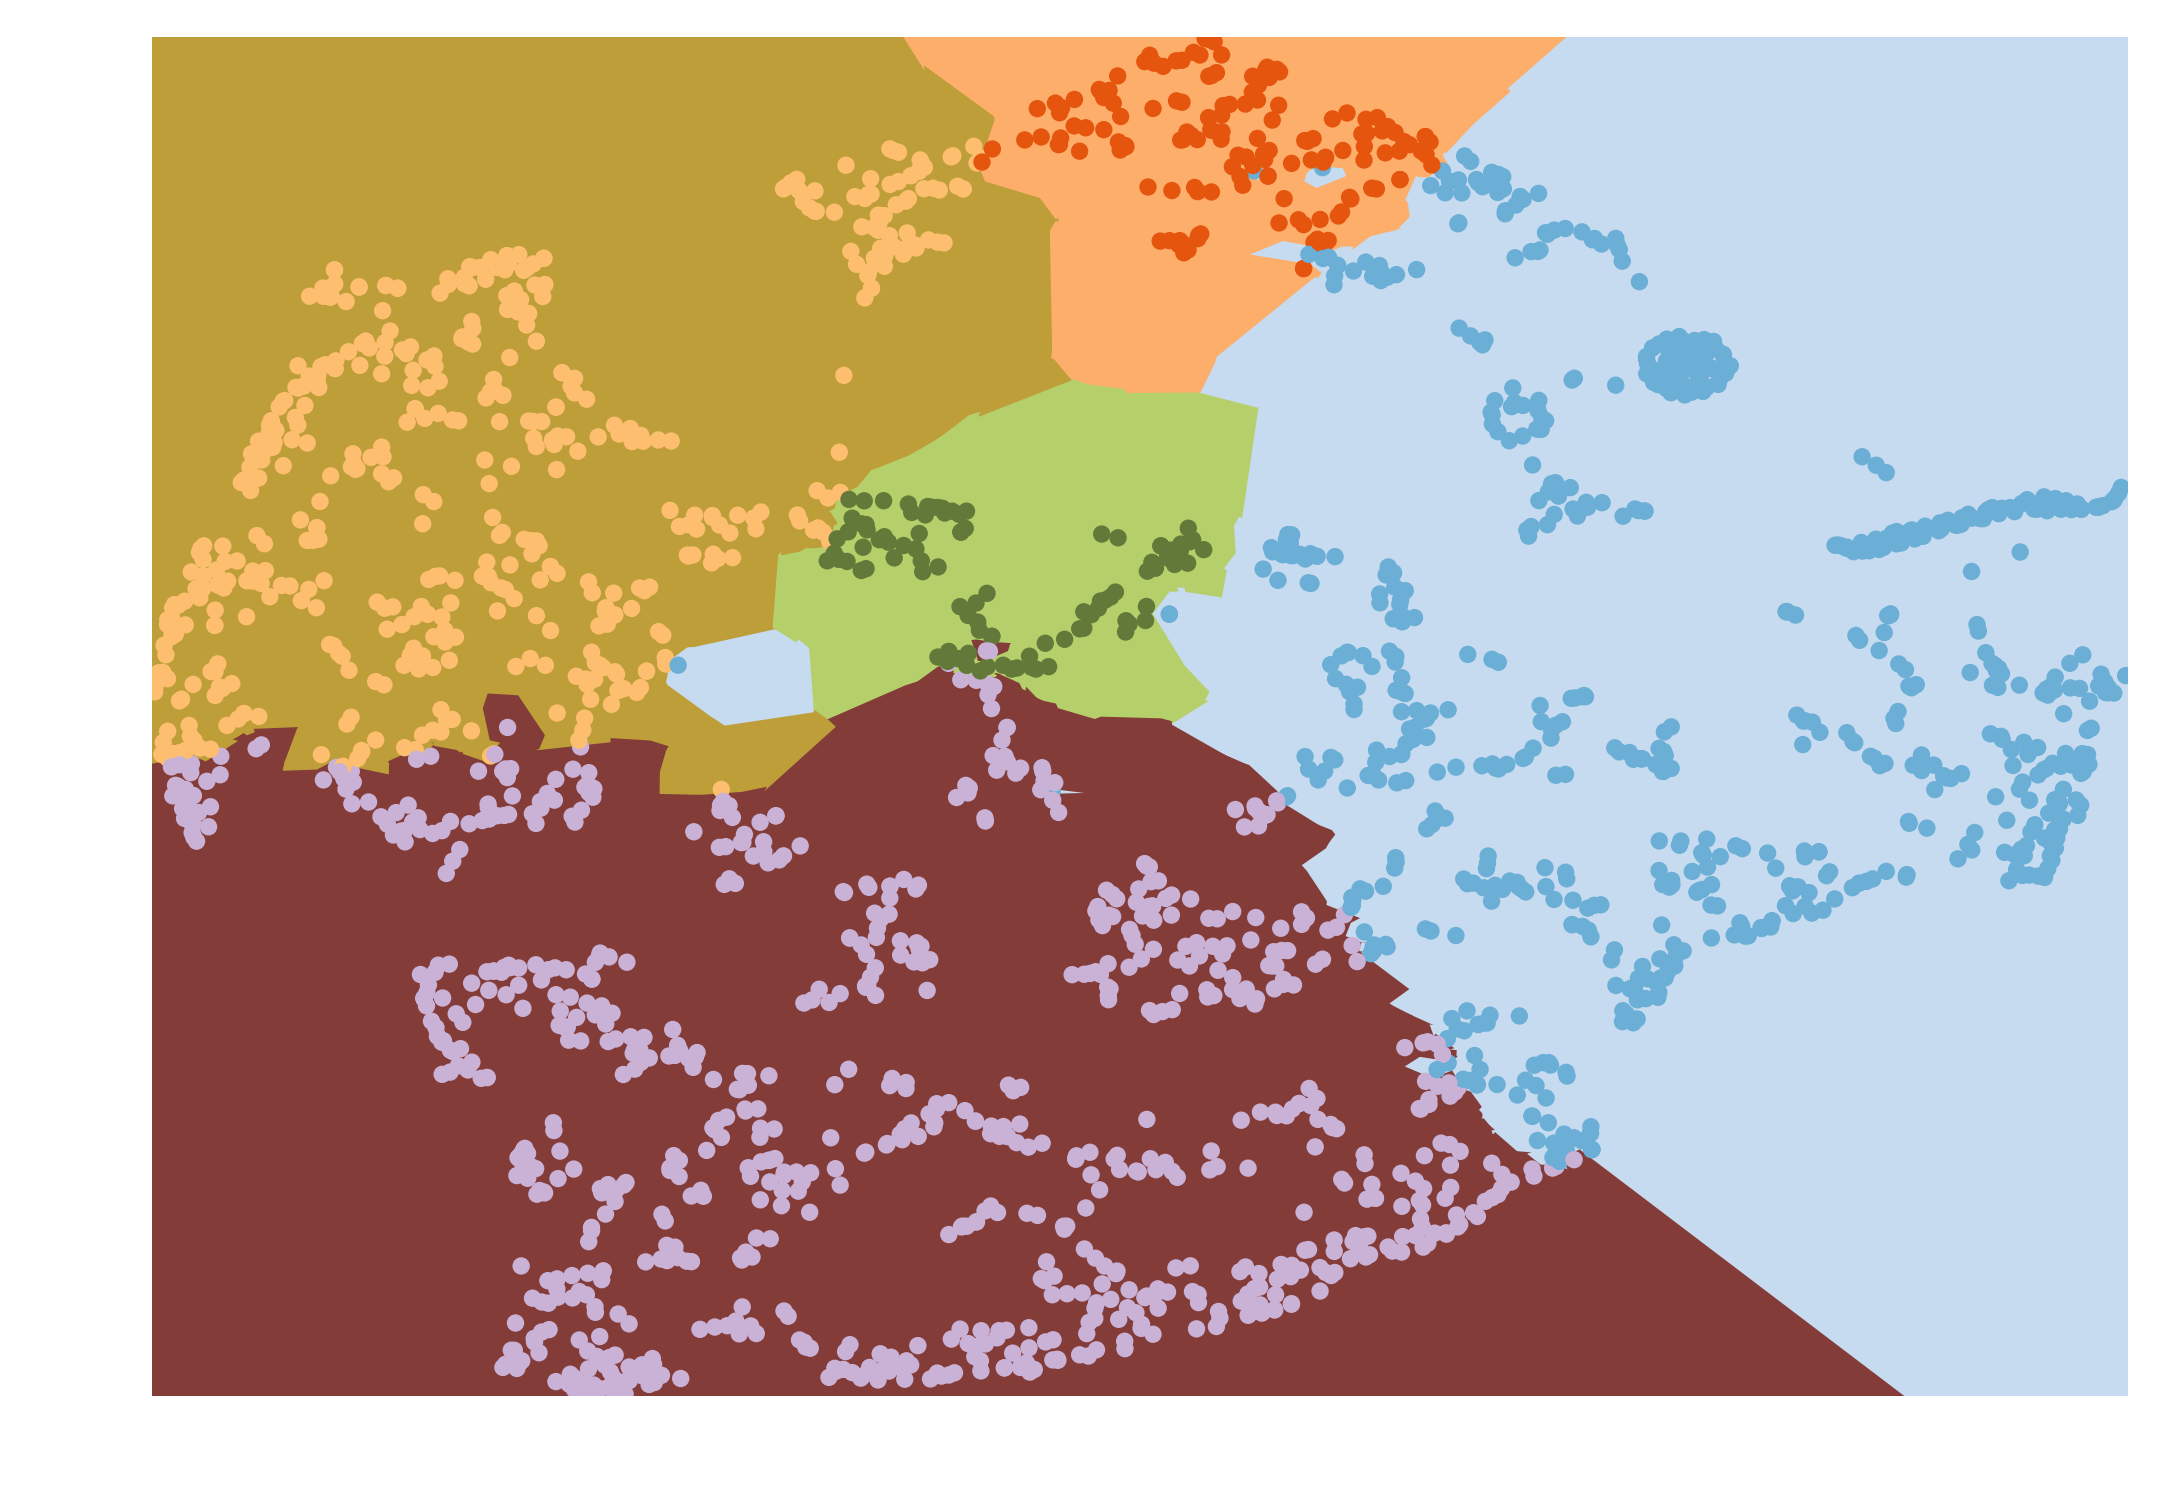
\includegraphics[width=.8\textwidth]{static/topics_5.png}
%     \end{center}
% \end{frame}

\begin{frame}
    \begin{center}
        \LARGE{\textbf{Is the Prisoner's Dilemma a collaborative field?}} \\ \vspace{.6cm}
        
\includegraphics[width=.15\textwidth]{static/detective.png} \\ \vspace{.5cm}
    \end{center}
\end{frame}

\begin{frame}
    \begin{center}
    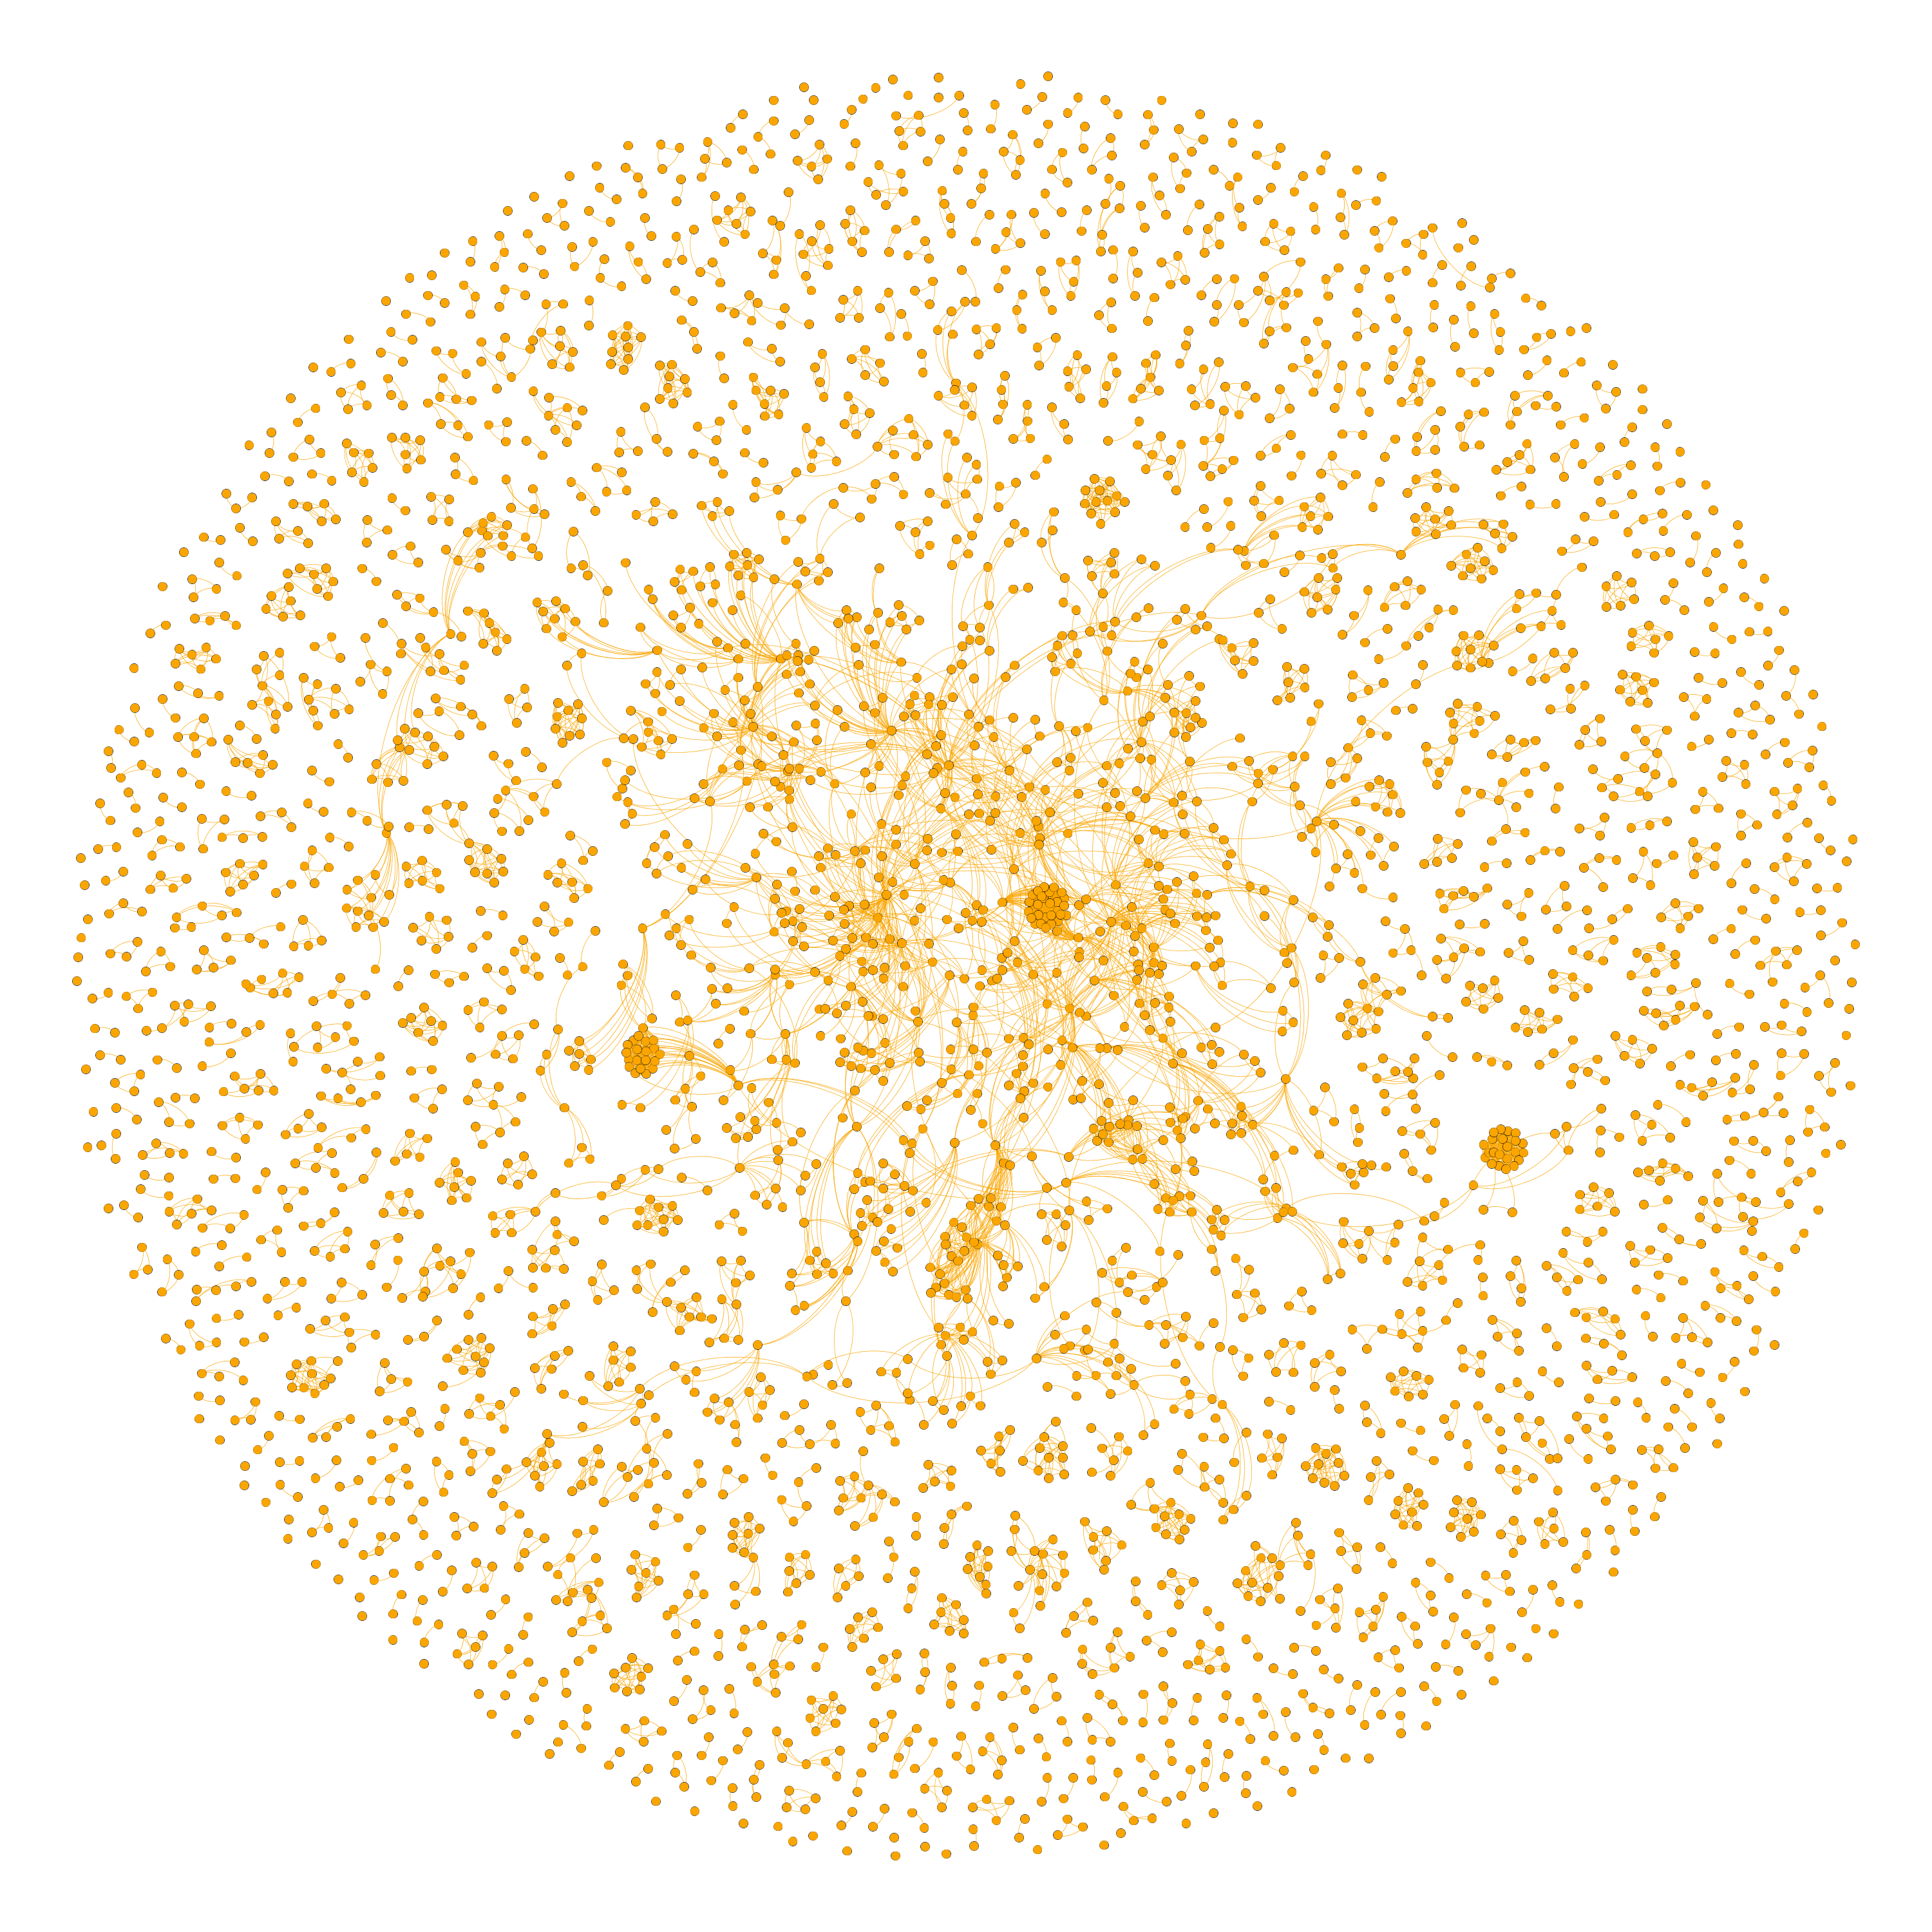
\includegraphics[width=.7\textwidth]{static/pd.png}
    \end{center}
\end{frame}

\begin{frame}
    \begin{center}
    
\includegraphics[width=.7\textwidth]{static/degree_dist.png}
    \end{center}
\end{frame}

\begin{frame}
    \begin{center}
        \large{``A bibliometric study of research topics, collaboration and influence in the field of the Iterated Prisoner's Dilemma"} \\ \vspace{.5cm}
        \small{Nikoleta E. Glynatsi, Vincent A. Knight} \\ \vspace{.5cm}
        \small{https://arxiv.org/abs/1911.06128}
    \end{center}
\end{frame}

\begin{frame}
    \begin{center}
    \faTwitter @NikoletaGlyn \\
    
    \vspace{1cm}
    \end{center}

    \footnotesize
    \faTwitter @drvinceknight \\
    $\bullet$ \url{https://nikoleta-v3.github.io} \\
    $\bullet$ \url{https://arxiv.org/abs/1911.06128} \\
    \faGithub  \ \url{https://github.com/Nikoleta-v3/bibliometric-study-of-the-prisoners-dilemma} \\
    \faGithub  \ \url{https://github.com/ArcasProject/Arcas} \\
    $\bullet$ \url{https://nikoleta-v3.github.io/2019/06/women-publications-in-mathematics.html} \\
    $\bullet$ \url{http://iltabiai.github.io} \\
\end{frame}

\end{document}

